\documentclass{article}
\usepackage[screen]{geometry}
\usepackage{alltt,xcolor}
\usepackage[utf8]{inputenc}
\usepackage{listings}
\usepackage{graphicx}
\lstset{escapechar=\@,language=C++,keywordstyle=\color{blue},showstringspaces=false}
\begin{document}
\large 
\section*{Specification}
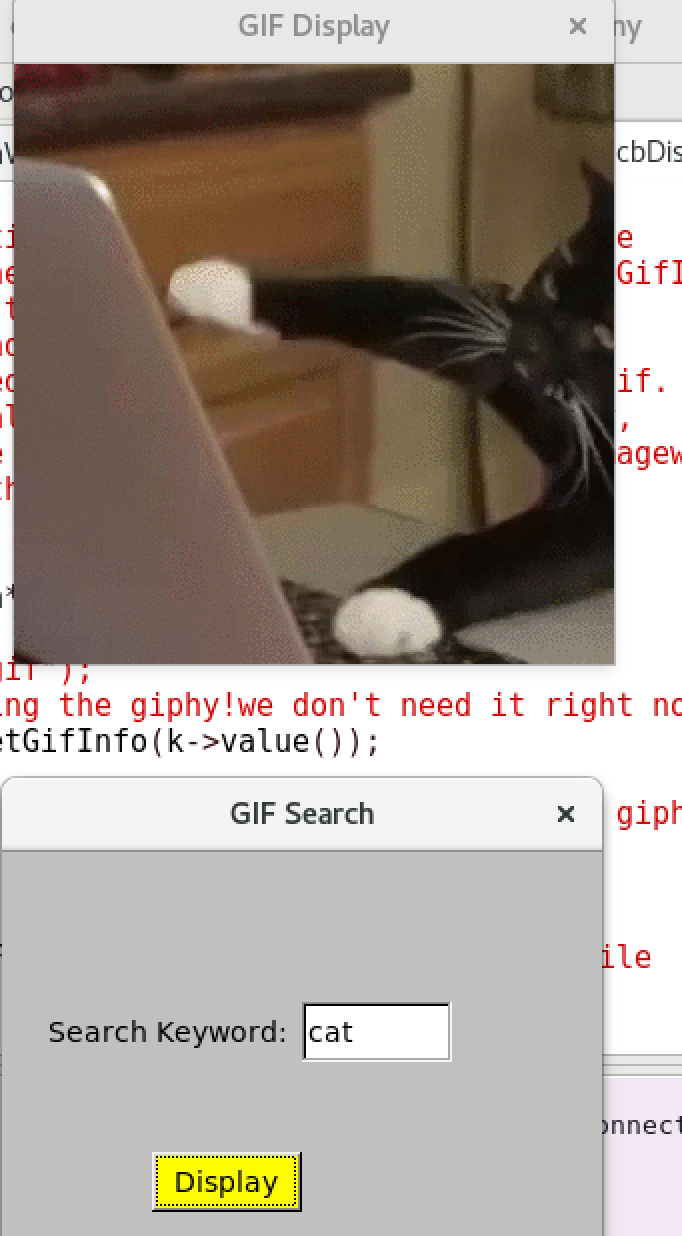
\includegraphics[width = 7cm, height = 11cm]{cat.png}
\begin{description}
	\item Search for a gif file related to a keyword the user types into a GUI textboxand display it in a separate window. 
\end{description}
\newpage\section*{Analysis}
\begin{description}
	\item [Inputs]  A keyword entered into a textbox
	\item [Process]  Send query to mashape giphy API to retrieve information about a gif matching the user’skeyword.  Parse the info to find a single gif to download using wget program.
    \item [Outputs]  A gif image related to the keyword
\end{description}
\newpage\section*{Design}
\begin{description}
	\item [main]  Call functions makeSearchWindow and makeDisplayWindow
	\item [getGifInfo]  Call searchGiphy to get information about gif from mashape
    \item [searchGiphy]  libcurl interface to communicate with internet
    \item [makeSearchWindow]  Create window to get input from user
    \item [makeDisplayWindow]  Create window to display the gif image
    \item [cbDisplay]   Callback function when user clicks button to call getGifInfo and put returned gif image inbox for display
\end{description}
\newpage\section*{Implementation}
\lstinputlisting{Makefile}
\lstinputlisting{main.cpp}
\lstinputlisting{makeSearchWindow.cpp}
\lstinputlisting{makeDisplayWindow.cpp}
\lstinputlisting{cbDisplay.cpp}
\lstinputlisting{getGifInfo.cpp}
\lstinputlisting{searchGiphy.cpp}
\newpage\section*{Test}
\subsection*{Testcase 1}
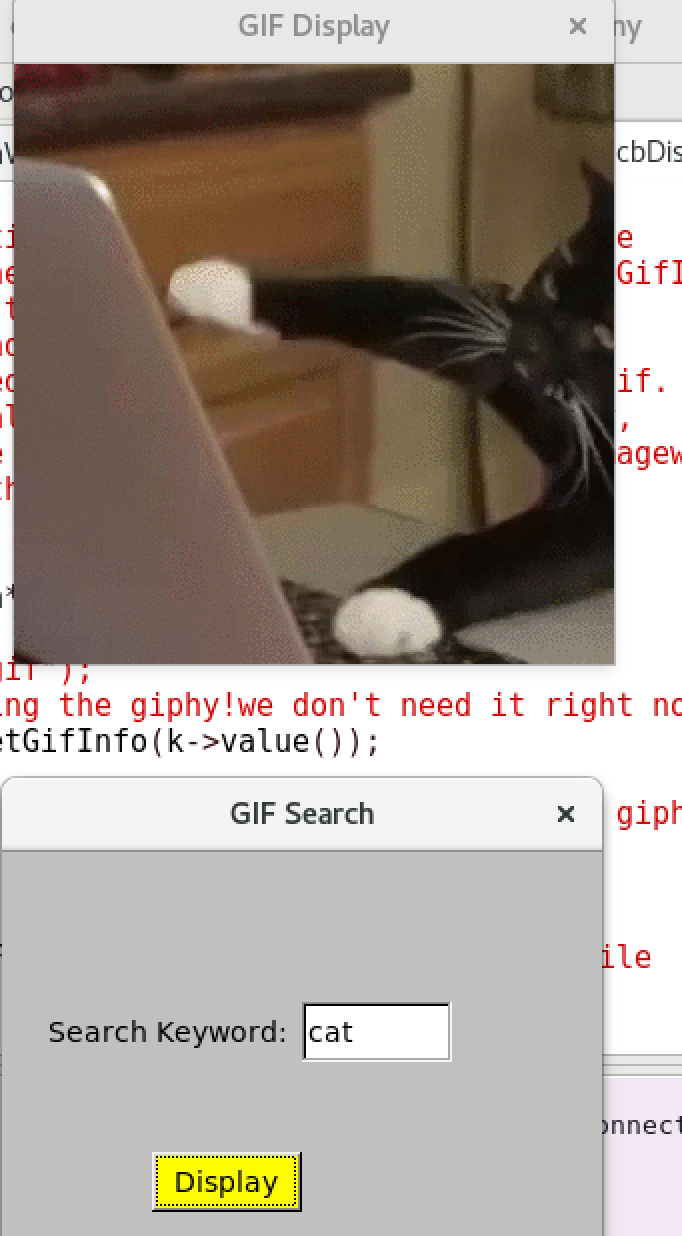
\includegraphics[width = 6cm, height = 9cm]{cat.png}
\begin{description}
	\item When the user typed cat as the key word, the program 
	will show the user the cute cat.
\end{description}
\newpage
\subsection*{Testcase 2}
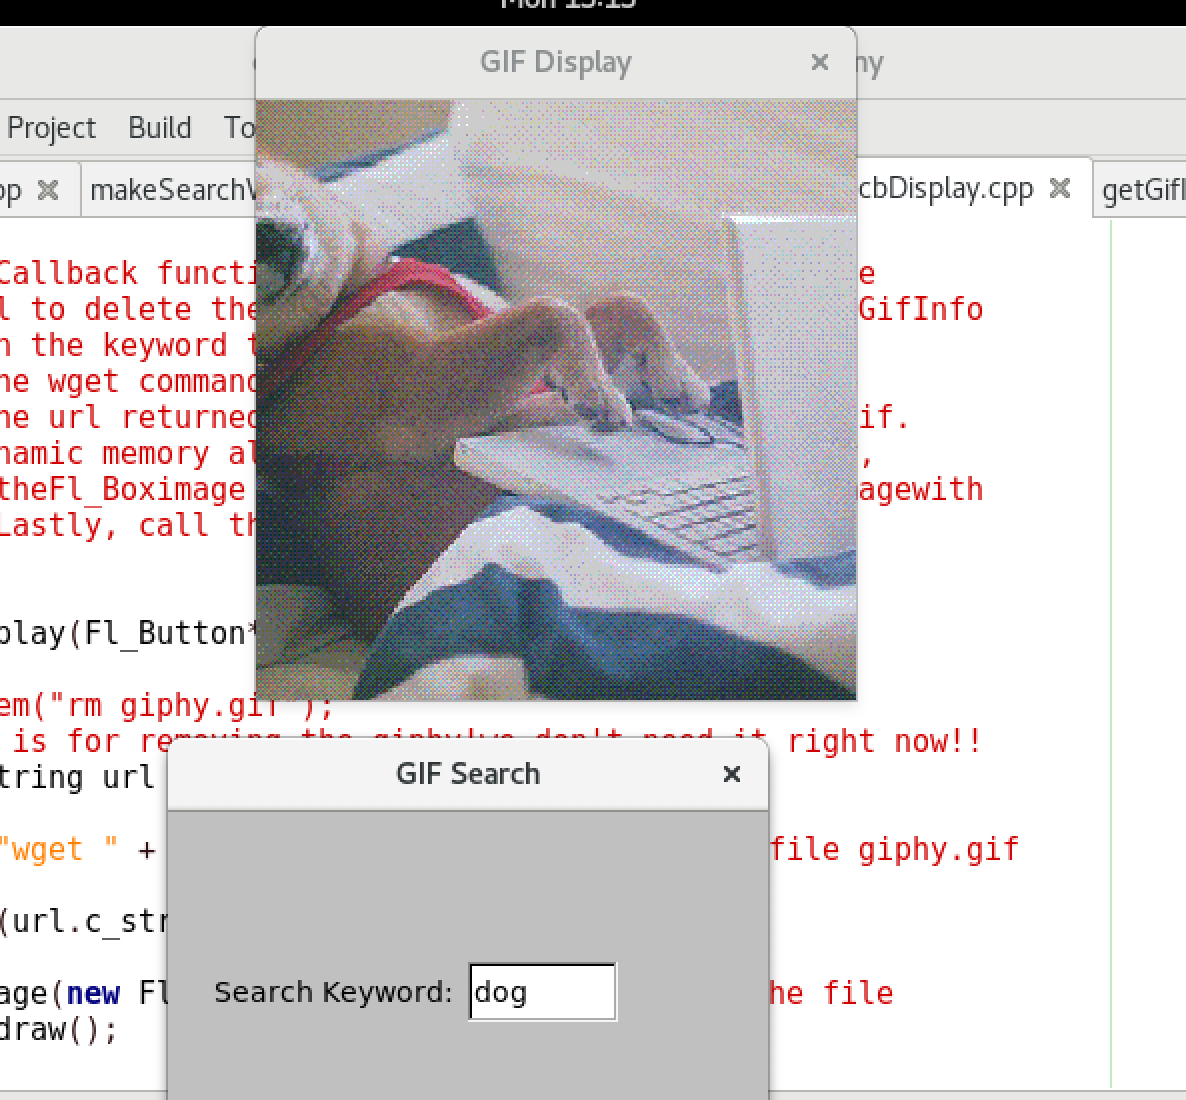
\includegraphics[width = 9cm, height = 8cm]{dog.png}
\begin{description}
	\item When the user typed dog as the key word, the program 
	will show the user the lovely dog.
\end{description}
\newpage
\subsection*{Conclusion of my testcases}

\includegraphics[width = 10cm, height = 9cm]{happy.png}
\begin{description}
	\item As we can see in my testcases, all of my codes run well.
	\item I successfully acheived the goal of this lab assignment!
\end{description}
\end{document}
